\documentclass[11pt,a4paper]{article}
\usepackage[margin=24mm]{geometry}
\usepackage[T1]{fontenc}
\usepackage{lmodern,microtype,amsmath,booktabs,array,graphicx}
\usepackage[numbers,sort&compress]{natbib}
\usepackage[hidelinks]{hyperref}
\usepackage{xurl}
\newcommand{\doi}[1]{\url{https://doi.org/#1}}
\setlength{\parindent}{0pt}
\setlength{\parskip}{5pt}
\setlength{\emergencystretch}{2em}
\renewcommand{\arraystretch}{1.15}
\makeatletter
\setlength{\@fptop}{0pt}
\setlength{\@fpsep}{18pt}
\setlength{\@fpbot}{0pt plus 1fil}
\makeatother
\title{Context Controls and EEG Pairing in Retrospective Valence Prediction: An Exploratory FACED Study}
\author{Muhammad Muntazar \and Muhammad Wasif Shakeel}
\date{National University of Sciences and Technology (NUST), Islamabad, Pakistan}
\begin{document}
\maketitle
\begin{abstract}
\textbf{Purpose.} To evaluate whether tested EEG recipes improve individual retrospective valence prediction beyond supplied elicitation metadata on FACED.
\textbf{Methods.} Seventy source and twenty development-validation participants formed three overlapping title-held rotations. Category and metadata controls, spectral regression and EEGNet residual prediction were examined with acquisition fallback and constrained EEG swaps. Subsequent source diagnostics assessed late versus distributed spectral coverage on 840 held pairs and longer EEGNet learning on one 84-pair panel. All evaluations reused development data; 33 reserved participants remained sealed.
\textbf{Results.} Mean unfamiliar-title validation MAE was 1.2602 for category medians, 1.2156 for spectral/context prediction and 1.2550 for EEGNet/context prediction; all corresponding gain intervals included zero. In the later source comparison, distributed spectral MAE was 1.4455 versus 1.3665 for matched context. On the separate neural panel, fixed 360-epoch EEGNet MAE was 1.4075 versus 1.2953 for context and 1.0994 for category medians. Source error continued decreasing; real and shuffled small-set targets were fitted.
\textbf{Conclusion.} Basic learning capacity does not establish incremental EEG utility. These adaptive evaluations support a bounded case study, without establishing convergence, equivalence to context or absence of affective EEG information. Credible comparator qualification and independent replication remain necessary.
\end{abstract}
\noindent\textbf{Keywords:} EEG; valence regression; stimulus context; FACED; participant generalization; exploratory evaluation

\section{Introduction}
EEG emotion benchmarks often predict assigned stimulus categories, whereas individual affect can differ within a stimulus. FACED provides elicitation categories and retrospective individual ratings \cite{chen2023faced}. Predicting individual valence requires testing whether EEG adds information beyond supplied experimental context.

Gerster et al. investigate FACED stimulus confounding \cite{gerster2026stimulus}; their later code includes individual categorical targets, clip-held evaluation and nested tuning \cite{gerster2026code}. Preprint/code version equivalence remains unverified. Other work examines video/time priors and shared versus individual continuous affect \cite{kong2026priors,wang2026shared}. HEART combines continuous valence--arousal--dominance regression with categorical prediction on FACED \cite{fernandez2026heart}; its correspondence to our item-10 target and catalogue-held evaluation remains unverified. We claim neither the first context control nor a novel architecture.

We ask whether the tested recipes improve individual retrospective valence prediction on new people and held catalogue titles. The exploratory contribution is an evaluation connecting category-supported controls, operational acquisition fallback, pairing diagnostics and source learning-capacity checks. EEGNet supplies an established compact backbone \cite{lawhern2018eegnet}, rather than a fully optimized or strongest-field decoder.

\section{Methods}
\subsection{Target, population and evidence blocks}
The outcome is FACED item-10 post-clip valence, with negative-to-positive anchors on 0--7. All endpoints and midpoint ratings are retained. Metadata exclusions and participant/material reservations preceded rating decoding. Neutral clips 13--16 share \emph{Blue} and are outside this non-neutral population; clip 22 is excluded because marker-duration and footage correspondence remain unresolved.

Seventy source, twenty development-validation and 33 reserved people are disjoint. Fourteen title families enter development; eight others remain reserved. \emph{Unfamiliar} means absent from a fit's source-title catalogue, without certifying personal unfamiliarity or distinct physical footage. Three evidence blocks remain separate:

\textit{Earlier validation:} three overlapping rotations fit eight source titles (560 trials) and assess six held titles on twenty validation people (120 trials each). A familiar-title arm adds 160 trials per rotation. Source fitting has one title per category, confounding category and title.

\textit{Later spectral source comparison:} five participant folds crossed with two material assignments produce ten cells, each with 448 training trials (56 people/eight titles) and 84 held trials (14 people/six titles). These yield 840 unique held pairs from seventy source people and twelve titles.

\textit{Later neural source diagnostic:} one metadata-first quality-complete cell uses the same 448/84 geometry, with different source people and disjoint titles across its partitions. Availability selection was label-blind but limits representativeness. It is neither an all-fold neural study nor new validation evidence. All held-material arms cover six categories; Fear and Inspiration are training-only.

\subsection{Processing and acquisition availability}
Headers calibrate signed ADC counts to microvolts at native 250/1,000 Hz. Trial-local processing uses common-average reference, a 50-Hz notch, 0.5--45-Hz forward/backward filtering and resampling to 128 Hz. A late 32-second interval ending at the recorded end marker supplies a trimmed 28-second core of seven four-second windows on thirty channels. This offline, acausal interval predicts whole-clip retrospective valence.

Fixed engineering rules assess rails, stuck counts, amplitude, line power and numerical validity; at most three channels permit spherical-spline repair \cite{perrin1989spherical}. All 980 source late intervals pass after repair. Fifteen of 280 validation trials lack available EEG, fourteen belonging to one person. All remain scored using the declared historical fallback. This policy followed earlier development inspection.

The later coverage comparison adds early/middle regions with the same processing. Their trimmed cores overlap; distributed features do not represent an entire film. Common availability requires all three regions to pass, leaving 979 source trials available and one middle-region failure. All 980 source trials remain eligible for fitting: EEG features missing by policy receive available-training-donor means. Both joint models and matched context share category fallback at inference; the actual 840 held pairs all have EEG. Thus matched context uses an EEG-availability route, whereas category median is the practical acquisition-free comparator. Thresholds remain fixed across the later comparison.

\subsection{Predictors, selection and learning}
Context comprises eight category and three acquisition indicators, catalogue duration and presentation ordinal. No evaluated person's rating or held-title rating consensus is supplied. Five-band log power averaged across seven windows gives 150 EEG features. Distributed coverage averages the early/middle/late log-feature vectors, preserving dimension.

An initial source-selection diagnostic jointly withheld the only source title for a category and therefore removed held-category support. Revised five-fold participant-held selection preserves every source category and compares global/coarse/category medians and category/full-context Ridge. Category median wins every rotation; both Ridge controls select alpha 0.1 from five candidates. This qualifies prediction on source titles, without certifying unfamiliar-title transfer.

Earlier spectral/context Ridge retains alpha 100. Earlier EEGNet-8,2 uses a local scalar head, participant-excluded context residuals, one loss per original trial after averaging seven window outputs, and a two-initialization ensemble. Twenty fits test bounded schedules through 120 epochs; rotation-0 validation selects schedules transferred to rotations 1/2. The retrospective alpha-100 context sensitivity shares the historical joint fallback, making feature-addition gain exactly zero on unavailable inputs. Pairing diagnostics exchange EEG between people sharing title/acquisition group, or titles sharing person/coarse valence; recipient context remains fixed. Thirty-two constrained derangements retain every recipient, including ineligible cases.

The later source coverage study tests Ridge alpha 0.1/10/100. A symmetric shared-alpha rule nominates 100 and distributed coverage, without independently optimizing context. The separate neural diagnostic fixes alpha-100 context, four participant-excluded inner folds for training offsets, source-only channel scaling and the 1,841-parameter scalar EEGNet adapter. Two initializations train 360 epochs at learning rate 0.001, AdamW weight decay 0.01, dropout 0.5 and original-trial batch eight. Epochs 120/240 are diagnostics; 360 is the fixed primary endpoint. Two 200-epoch capacity controls use the same 32 training trials with real or one fixed permutation of targets, without held evaluation. MSE training and MAE assessment target different losses.

\subsection{Endpoints, uncertainty and verification}
Predictions average across initializations before clipping to 0--7. MAE equally weights people and title families. Gain is comparator minus EEG-recipe MAE; pairing change is swapped minus original MAE. Rotation averages summarize dependent panels.

Earlier paired participant/title bootstrap intervals use 4,000 draws. They are descriptive on reused outcomes, without selection or multiplicity adjustment \cite{owen2007,owen2012}; six held titles limit precision \cite{westfall2014power}. Later source scores are descriptive CV/cell summaries, without confirmatory intervals. Independent numerical audits verify exported losses, identities and offsets. Checkpoint reloads verify fixed source/held forward subsets, without independently replaying every waveform or scaler moment. No protected outcomes support any result.

\section{Results}
\begin{table}[tbp]
\centering
\small
\caption{Unfamiliar-film validation MAE on the original 0--7 rating scale (lower is better).}
\label{tab:primary}
\begin{tabular}{lrrrr}
\toprule
Predictor & R0 & R1 & R2 & Mean \\
\midrule
Category median (source selected) & 1.222 & 1.232 & 1.327 & 1.260 \\
Category Ridge (source selected) & 1.252 & 1.234 & 1.315 & 1.267 \\
Full-context Ridge (source selected) & 1.253 & 1.220 & 1.338 & 1.270 \\
Matched context, $\alpha=100$ (sensitivity) & 1.258 & 1.210 & 1.311 & 1.260 \\
Spectral + context Ridge (frozen) & 1.259 & 1.177 & 1.211 & 1.216 \\
EEGNet + context residual (frozen) & 1.191 & 1.311 & 1.263 & 1.255 \\
\bottomrule
\end{tabular}
\par\medskip\begin{minipage}{0.97\linewidth}\footnotesize Each panel contains 20 held people and six title families; all outcomes, including unavailable EEG, are retained. The mean is a descriptive average of dependent rotations. Category/full-context selection is source-person-only and familiar-title CV; frozen EEG recipes were previously development selected. Matched context is a separately declared retrospective sensitivity with the historical joint fallback shared by both methods on acquisition failures.\end{minipage}
\end{table}


Against category medians, earlier spectral/context unfamiliar-title gains are \(-0.0368\), \(+0.0549\) and \(+0.1158\), averaging 0.0446; EEGNet gains average 0.0052 (Table~\ref{tab:primary}). All six gain intervals include zero. Matched-context spectral gains average 0.0440, with all three intervals including zero. Familiar-title mean MAEs are 1.1723 (category), 1.2094 (spectral/context) and 1.2918 (EEGNet/context). EEGNet's adverse rotation-2 familiar gain is \(-0.1852\), interval \([-0.3498,-0.0143]\). Historical conditions remain in the supplement.

\begin{figure}[tbp]
\centering
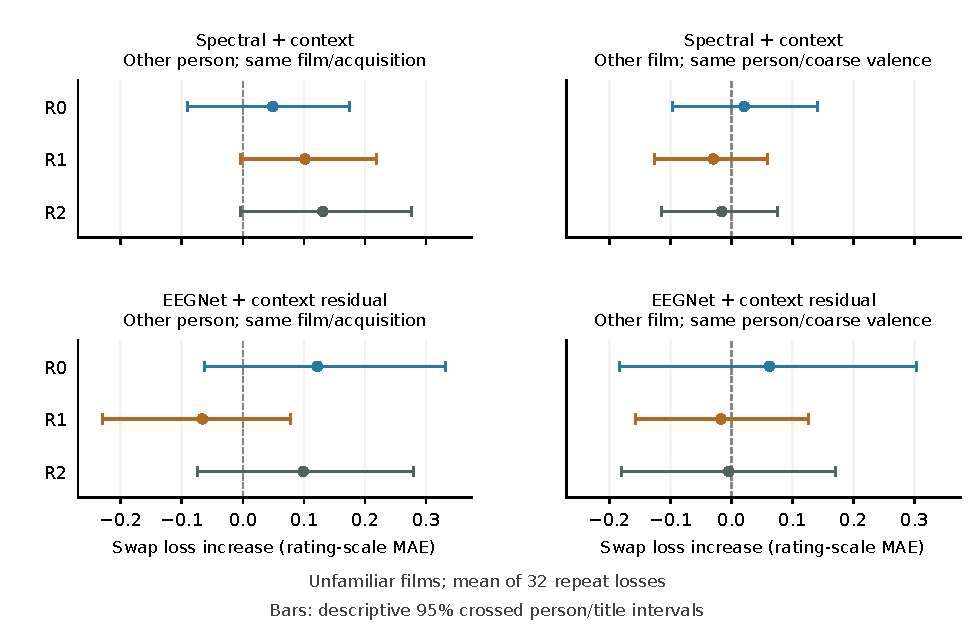
\includegraphics[width=\linewidth]{figures/pairing_publication.pdf}
\caption{Earlier unfamiliar-title pairing diagnostics. Positive change means swaps raise MAE. Points average 32 repeat losses; bars are descriptive crossed participant/title intervals. Ineligible and unavailable recipients remain unchanged. All twelve displayed intervals include zero; the supplement retains all twenty-four panels.}
\label{fig:pairing}
\end{figure}

\begin{samepage}
Same-title person swaps raise unfamiliar spectral MAE by 0.0487/0.1017/0.1309; EEGNet changes are 0.1221/\(-0.0665\)/0.0987 (Fig.~\ref{fig:pairing}). Same-person title swaps have smaller, mixed changes. All twenty-four pairing intervals include zero. Additive title terms account for 43.3\%/42.3\% of source/validation squared rating deviations; these descriptive components do not identify a decodable neural residual.
\end{samepage}

\begin{table}[tbp]
\centering\small
\caption{Later source diagnostics, separate from the earlier validation panels.}
\label{tab:sourcefollowup}
\begin{tabular}{lrrr}
\toprule
\multicolumn{4}{l}{A. Spectral comparison: 840 held pairs across ten source cells}\\
Predictor & \multicolumn{3}{r}{Held MAE}\\
\midrule
Category median & \multicolumn{3}{r}{1.3040}\\
Matched context, $\alpha=100$ & \multicolumn{3}{r}{1.3665}\\
Late EEG + context, $\alpha=100$ & \multicolumn{3}{r}{1.4646}\\
Distributed EEG + context, $\alpha=100$ & \multicolumn{3}{r}{1.4455}\\
\midrule
\multicolumn{4}{l}{B. EEGNet diagnostic: 84 held pairs in one reused source cell}\\
Epoch & Source MSE, seed 1 & Source MSE, seed 2 & Held MAE\\
\midrule
120 & 1.3416 & 1.3966 & 1.3769\\
240 & 0.9921 & 1.0956 & 1.3759\\
360 (fixed primary) & 0.8647 & 0.8783 & 1.4075\\
\midrule
Category median & \multicolumn{3}{r}{1.0994}\\
Matched context, $\alpha=100$ & \multicolumn{3}{r}{1.2953}\\
\bottomrule
\end{tabular}
\par\medskip\begin{minipage}{0.97\linewidth}\footnotesize Lower is better. Each source cell fits 448 trials and assesses 84 participant/title-held trials. Panel B is one metadata-selected complete cell, not the neural counterpart of all ten panel-A cells. Source MSE uses unbounded eval-mode predictions with training offsets; held MAE clips the two-seed mean. No score is independent confirmation, and no confidence interval is inferred across these overlapping fits.\end{minipage}
\end{table}


The later spectral comparison is adverse against both controls (Table~\ref{tab:sourcefollowup}A). Distributed coverage improves on late-only MAE by 0.0191 at alpha 100, while trailing matched context by 0.0790 and category medians by 0.1416. All tested EEG/alpha combinations trail their matched context and category comparators. Context's lowest tested MAE is 1.3450 at alpha 0.1; the shared-alpha control is therefore not its individually best setting.

On the separate neural cell, both source trajectories learn substantially: final source MSE falls 71.5\%/71.0\% from offset-only error 3.0314. Yet the fixed 360-epoch held MAE is worse than context/category by 0.1121/0.3081; earlier checkpoints also trail both. Between epochs 240 and 360, eval-mode source MSE falls another 12.8\%/19.8\%; an optimization plateau is unestablished. The 32-trial real/shuffled capacity errors fall from 6.1130 to 0.1058/0.1397. Arbitrary-target fitting establishes small-set learning capacity, without establishing emotion information or full-set interpolation.

\section{Discussion}
Category-supported selection corrects an information mismatch and supplies a competitive simple comparator. The earlier small favorable average spectral gain is not consistent across rotations. Later source results provide no incremental lead for either the distributed spectral recipe or the tested longer neural schedule. These evaluations differ in people, titles, fitting size and adaptive history; their errors cannot be pooled or read as a controlled before/after improvement.

Small-set fitting narrows a basic implementation/learning concern. Continued source improvement alongside adverse held prediction is compatible with overfitting or poor transfer, without identifying its cause. Additional epochs could lower training error without improving utility. MSE/MAE mismatch, fixed regularization, one neural cell and incomplete stronger-method qualification limit an optimized-null interpretation. Pairing dependence can reflect acquisition, artifacts or identity; swaps do not isolate emotion-specific or causal cerebral information.

Other limits are a single corpus, one retrospective rating per cell, six held categories, few title families, supplied context, overlapping EEG cores and unauthenticated footage/playback timing. Common QC routing makes the late/distributed comparison about representations, not recording cost. Held missing-input behavior is not empirically tested by the later source panel. Adaptive exploration, overlapping rotations and reused outcomes preclude independent confirmation. HEART's exact target correspondence remains unresolved; neither priority nor state-of-the-art superiority is claimed.

All 33 reserved participants remain sealed. Source and manufactured-input export checks qualify implementation, without supplying replication or novelty. Stronger claims require credible comparator qualification and independent participant/material evidence under a fixed protocol.

\section{Conclusion}
The tested EEG recipes do not establish consistent incremental valence prediction beyond context. Learning-capacity controls and longer source training clarify this bounded finding without establishing convergence, equivalence or a general absence of EEG information. The released evaluation preserves acquisition failures, adverse results and the boundary between development and independent confirmation.

\section*{Declarations}
This secondary analysis collected no new recordings. FACED reports original ethics and consent \cite{chen2023faced}; that approval does not establish a new institutional exemption. Anonymous development predictions, code and audits are available at \url{https://github.com/Overproness/GRU-XNet_EEG_Emotion_Recognition}; original recordings, rating archives and private checkpoints are not redistributed. Generative-AI assistance supported drafting, code preparation and checking; the authors remain responsible.

\bibliographystyle{unsrtnat}
\begingroup
\interlinepenalty=10000
\small
\setlength{\bibsep}{3pt}
\bibliography{references}
\endgroup
\end{document}
